\section{Første iteration}

Formålet med elaborationsfasen er at skabe en interaktiv udvikling af produktet MMMI´s\footnote{{mangfoldig manager management instruments}} funktionalitet. Denne udvikling sker på baggrund af inceptionsfasen\footnote{{Bilag : Inceptionss dokumentet}}, hvor der blev opstillet en række krav til MMMI-projektet.  For at kunne nå de mål bliver der lagt lavet nogle mindre iterationer her under krav, analyse, design, kode og test som arbejdes med ud fra de overordnede kravspecifikationer. Målet er at får en funktionel kode færdig til elaborationsmilepælen. 


\section{Analyse}
Der er blevet lavet en række diagrammer over de forskellige detaljeret brugsmønster.\\
Der er to forskellige typer af analyse diagrammer, der er de dynamiske og de statisk.
\subsection{Statiske side af analysen}
\begin{figure}
  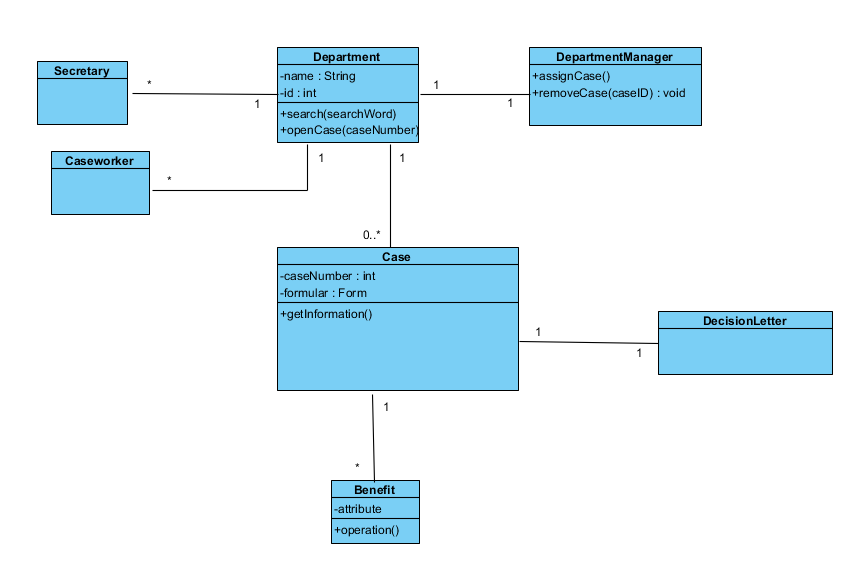
\includegraphics[width=\linewidth]{./PNG/analyseKlasseDiagram.PNG} 
  \caption{Analyse klasse diagram.}
  \label{fig:AKlasse}
\end{figure}



\subsection{Design}
\subsubsection{DesignStatisk}
\begin{figure}[h]
\includegraphics[width = \linewidth]{./PNG/design/designKlasseDiagram.PNG}
\caption{Klasse diagrammfuld størrelse se interne bilag afsnit \ref{sec:diverse} figur \ref{fig:fuldDesignKlasseDiagram}}
\label{fig:desginklasse}
\end{figure}
Diagrammet \ref{fig:desginklasse} beskriver de klasser vi har fundet, der skal implementeres i systemet. Hver klasse har attributter og en del skal have skrevet getter / setter-metoder til, men for at diagrammet ikke skal blive for stort og uoverskueligt, blev der valgt at undlade dem.\\
Diagrammet er blevet designet med tanker på en tydelig lagdeling og repræsentere systemets domænelag. Der blev besluttet at ”Department”-klassen skulle benyttes som facadeklasse til præsentationslaget, mens datahandler interfacet bruges til kommunikation mellem domæne- og persistentslag.
Department – Facade klasse\\
Der var særligt fokus på attributterne: ”id” af typen int og ”caseMap” af typen Map<String, Case>. Det var tænkt at ID skulle bruges til at godkende adgangen til sager i databasen, for at imødekomme projektets ”Dataafgrænsning”. ID er af typen int, for at holde den simpel. Kravet til dataafgrænsningen er, at en arbejder der henter information omhandlende en borger, ikke må blive gjort opmærksom om sager, der administreres af andre afdelinger end arbejderens egen.\\
Tanken bag attributten ”caseMap”, var at department skulle have en liste af case-objekter som kunne bruges til at hente de relevante informationer frem for at sende dem til præsentationslaget. Der blev valgt at bruge et Map da Key/Value-strukturen gør det nemmere at finde en sag. Den Key der blev valgt til caseMap er caseNumber og skal bruges til metoden openCase(…)\\
Klassens metoder, som ”search(…)”, ”openCase(…)”, mm. er designet til at håndtere den logik, som controllerne fra præsentationslaget skal bruge. Metoderne repræsentere de funktioner som er ønsket i det grafiske userinterface (GUI).\\
Når metoden ”search(…)” kaldes, skal logikken først hente data fra persistenslaget. Dette sker gennem Interfacet PersistanceInterface som opretter et objekt af klassen ”SearchCase”, som er designet til at være en placeholder i domænelaget, for data der er relevant til en brugers søgeord.\\
\textbf{SearchCase – Placeholder klasse}\\
Klassen består af en constructor med attributterne: ”citizen”, ”caseNumber”, ”caseStatus”, ”date”, ”reason”, ”employeeName” og ”employeeID”. Disse informationer er ikke et udtryk for alt der ligger i en sag, men er nok til at præsentere en borgers sag og derefter hente de resterende informationer. \\
Hvis der er et ønske om at hente den fulde sag, gøres dette ud fra ”caseNumber”-attributten gennem ”openCase(…)” metoden, fra ”Department”-klassen . Den data der er relateret til en sag, hentes fra persistenslaget, gennem interfacet ”PersistanceInterfase”.\\
\textbf{PersistanceInterfase – Datahandler interface}\\
For at behandle dataflowet mellem persistenslaget og domænelaget, er der blevet designet et interface med metoderne: ”create()”, ”read()”, ”update()” og ”delete()”. Disse metoder blev valgt for at kunne lave, hente, ændre og slette data, som opbevares i persistenslaget. For at domænelaget kan sende dataforespørgsler til persistenslaget, skal der implementeres anonyme klasser af det påkrævede interface, som så kalder den ønskede interfacemetode.\\ 
\textbf{Case : Employee : Citizen – Objektklasser}\\
Objektklasserne blev designet med tanken om at præsentationslaget og persistenslaget, skulle arbejde med konkrete instanser af disse. Persistenslaget skulle tilføje den data, som var forbundet med objektet, som blev kaldt gennem domænelaget. Præsentationslaget skulle registrere indholdet i objekterne, pakke det ud og præsentere det som ønsket. \\
\textbf{JobTitle – Rollebaseret kontrol}\\
Superklassen ”JobTitle” blev designet til at kontrollere en given medarbejders rettigheder i systemet. Der blev taget udgangspunkt i tre jobstillinger, som blev skrevet op som subklasser - sekretær, sagsbehandler og afdelingsleder. Når en medarbejderklasse blev oprettet, skulle det være et krav, at de fik tildelt en stilling (JobTitle). Denne stilling skulle kunne ændre sig i systemet, f.eks. på grund af en forfremmelse, uden at medarbejderen skulle registreres på ny i systemet.\\
Stillingen som en medarbejder tildeles, skulle begrænse systemets funktionalitet, så de kun havde adgang til de områder, som var nødvendig til at udfører deres opgave. En sekretær skulle f.eks. ikke kunne andet end at registrere en person, som søger behandling samt årsagen for at der søges. En sagsbehandler skulle have fuld adgang til relevante sager, dvs. kun sager der er oprettet i den afdeling sagsbehandler er tilknyttet. En afdelingsleder skulle kunne det samme som en sagsbehandler, men også kunne styre hvilke sager de forskellige sagsbehandlere skulle arbejde på.\\
\textbf{Multiplicitet/Multiplicity – Klassernes forbindelser}\\
Forbindelserne mellem klasserne i designdiagrammet, består primært af aggregeringer. Klassen ”Employee” er forbundet med en many-to-one aggregering til klassen ”JobTitle”. Dette er blevet valgt, da objekter af klassen ”JobTitle” ikke skal blive slettet, hvis et ”Employee”-objekt fjernes. Tanken der ligger til grund for dette, er at ”JobTitle” kan være forbundet til flere forskellige ”Employee”-objekter. \\
Klassen ”Department” er forbundet til ”Employee” med to aggregeringer. Første aggregering er ”employeeList”, som er en one-to-many relation. Aggregeringen er blevet lavet, for at indikere at der kan være mange der arbejder i samme afdeling, men det skal stadig være muligt at slette en ”Department”, uden at slette ”Employee”-instanserne. Anden aggregering er ”departmentManager”, som er en one-to-one relation. Denne aggregering er blevet lavet, for at demonstrere at der altid skal være en leder i en afdeling. Igen skal det være muligt at slette en ”Department”, uden at det sletter ”Employee”.\\
Klassen ”Department” er forbundet til ”Case” med en enkelt aggregering. Dette er en one-to-zero-or-more forbindelse, som betyder at en afdeling ikke altid har nogen sager, men en sag er altid forbundet til en afdeling. Aggregeringen blev valgt, da en sag ikke forsvinder, hvis afdelingen bliver fjernet. \\
Klassen ”Case” er forbundet med to aggregeringer til klassen ”Citizen”, som også er forbundet med en komposition tilbage igen. Den første aggregering der er lavet, er en zero-or-many-to-zero-or-many relation, som omhandler en sags henvisning. En person kan blive henvist af nul eller flere personer, omhandlende det samme problem og på samme måde er det også muligt for en person at have henvendt sig for at få oprettet nul eller flere sager. Anden aggregering er lavet af samme grund som kompositionen er. En ”Citizen” kan have en til flere sager i gang på en gang, men en sag skal altid være angående en enkelt ”Citizen”. Aggregeringen er anvendt da det skal være muligt at fjerne en ”Case” fra systemet, uden at fjerne den ”Citizen” sagen omhandler. Kompositionen er derimod blevet brugt, da en ”Case” altid vedrører en ”Citizen”, og hvis denne fjernes fra systemet, skal de relaterede ”Case”-objekter fjernes, da de ikke længere vedrører nogen.\\
Klassen ”SearchCase” er forbundet med en komposition fra interfacet ”PersistanceInterfase”. Da et interface ikke kan instantieres, har det ikke nogen multiplicitet. Kompositionen er blevet valgt, da ”SearchCase” ikke fungere uden interfacet, og forsvinder derfor, hvis interfacet fjernes.\\


\subsection{DesignDynamisk}


\subsection{Implementering}
Målet med første iteration var at skabe et domain lag der havde de funktionalitetter som var nødvendige for systemet så det kunne fungere. Dette blev gjort så gruppen havde en bedre forståelse for hvordan systemet skulle se ud. I det følgende tekst er der lagt vægt på brugsmønsterende opret sag og find sag. Igennem første iteration var der lavet to klasse (case og department) der implementeret begge brugsmønster. ”case” håndteret hvad for noget data der skulle gemmes i en sag, mens ”department” holdt styr på hvad for nogle sager der var og hvordan man skulle finde dem.  Nedenfor ses de forskellige attributter der var I ”case” klassen(ref), udover dem var der gætter og sætter på attributterne. 
\\INSERT KODE\\
Der bruges et map til at holde den data der ændre og skrives ind, mens der er en status på om sagen er lavet, I gang eller færdig. Der er og kan kun være en person, sagen omhandler så der er simple variable, mens der kan være flere der fortæller det kan være en god ide at den her person for noget hjælp. Det gjorde at der skulle være en list over disse personer. \\
For at kunne se hvad der skrives ud I præsentationslaget går det igennem facaden som er afdeling. Det er også her at alle de forskellige sager vil være gemt I denne iteration. Der bliver genererer et sagsnummer hvor det også er tydeligt at se for os hvilken afdeling sagen tilhørere. \\ 
For at oprette en sag skal der bruges en person og oprette sagen på hvilket gør at funktionen skal enten få en person ind eller få information nok ind så den kan selv oprette den person sagen omhandler. Neden for er ses det hvordan dette er blevet håndteret(ref). 
\\INSERT KODE\\
Som det kan ses I koden nedenfor(ref) ses det hvordan klassen ”department” finder en sag den skal bruge en ”string” som kunne være CPR-nummer for personen den omhandlede, sagsnummeret for sagen og navnet på personen sagen omhandler. 
\\INSERT KODE\\
Som det kan ses I koden er der ikke blevet returneret en sag, men en list af sager. Dette er blevet gjort af flere årsager. Et par af de årsager er at en person kan have flere sager og mere end en person hedder det samme. Det kan også være en bruger af systemet ikke kender hele navnet så det skulle være muligt at få alle med fornavnet Anders tilbage, dette nåede ikke at blive implementeret I denne iteration. 



\subsection{Test}
\begin{figure}[hbt!]
\begin{lstlisting}
public static void main(String[] args) {
	while (!quit) {
                rollInfor();
                text = sc.nextLine().toLowerCase();

                switch (text) {
                    case "secretary":
                        Employee trine = detDepartment.createEmployee("trine", 
                        252525, "secretary");
                        commands(trine);
                        break;
                    case "caseworker":
                        Employee mads = detDepartment.createEmployee("mads", 
                        353535, "caseworker");
                        commands(mads);
                        break;
                    case "departmentmanager":
                        Employee martin = detDepartment.createEmployee("martin", 
                        262626, "departmentmanager");
                        commands(martin);
                        break;
                    case "quit":
                        System.out.println("Du quiter");
                        quit = true;
                        break;
                    default:
                        System.out.println(text + "Er ikke en kommando\n");
                        break;
                }
\end{lstlisting}
\caption{tekst under figuren}
\label{kode:1main}
\end{figure}
Der blev ikke lavet unit test på første iteration, da det ikke blev set som en nødvendighed. Det der blev fokuseret på var systemtest som skulle sikre at forståelsen med projektet og hvordan de forskellige brugsmønstre ville fungere i et færdigt system. Der blev fundet flere fejl/mangler igennem systemet. Vist på koden (Se figur \ref{kode:1main}) kan det ses at der bliver lavet en ny ”employee” hvilket skyldes det ikke var lavet så den kunne huske mere end en ad gangen. Det kan ses I figur \ref{kode:1commando} er det de forskellige kommandoer som kan bruges returneres det vil derefter testes om personen der er logget ind. \\
Dette blev den eneste rigtige test da dette kom ud på at få ideen til hvordan systemet skulle fungere helt på plads så databasen og præsentations laget kunne blive lagt på. 
\begin{figure}[hbt!]
\begin{lstlisting}
public static String loop() {
        while (true) {
            Scanner s = new Scanner(System.in);
            String t = s.nextLine().toLowerCase();

            switch (t) {
                case "back":
                    return t;
                case "create case":
                    return t;
                case "close case":
                    return t;
                case "add information":
                    return t;
                case "assign case":
                    return t;
                case "reassign case":
                    return t;
                default:
                    System.out.println(t + " Er ikke en kommando \n");
            }

        }
    }
\end{lstlisting}
\caption{loopet der ser om kommandoen kan er rigtig}
\label{kode:1commando}
\end{figure}
Dette blev den eneste rigtige test da dette kom ud på at få ideen til hvordan systemet skulle fungere helt på plads så databasen og præsentations laget kunne blive lagt på.
\newpage
